\documentclass[a4paper,11pt]{article}
\usepackage[utf8]{inputenc}
\usepackage[italian]{babel}
\usepackage{amsmath}
\usepackage{amsfonts}
\usepackage{amssymb}
\usepackage{physics}
\usepackage{graphicx}
\usepackage{subfigure}
\usepackage[italiano, ruled]{algorithm2e}
\usepackage[left=1in, right=1in]{geometry}

%opening
\title{Simulazione numerica di una particella libera sul cerchio nel limite di bassa temperatura}
\author{Rocco Francesco Basta}
\date{}

\newcommand{\avg}[1]{\langle {#1} \rangle}

\begin{document}

\maketitle

\begin{abstract}
    Lo studio numerico del sistema quantistico di una particella libera sul cerchio presenta particolari difficoltà dovute alla peculiare topologia del sistema. Sono stati messi a confronto tre diversi metodi per misurare la suscettività topologica del sistema nel limite di bassa temperatura: un algoritmo Metropolis locale, un algoritmo non locale e infine un metodo basato sullo studio di sottovolumi (\emph{slab}) del cammino totale. Infine, il metodo non locale è stato applicato allo studio dello spettro del sistema. 
\end{abstract}

\section{Introduzione}

    Il sistema è composto da una particella di massa $m$, libera di muoversi su un cerchio di raggio $R$. L'hamiltoniana del sistema è
    
    \begin{equation}
        H = \frac{p^2}{2m} \quad \quad p = \frac{\hbar}{i} \partial_x
    \end{equation}
    
    dove $x \in [0, L = 2\pi R)$. D'ora in poi, poniamo $\hbar = 1$.
    
    Per effettuare la simulazione, passiamo a quantità adimensionali:
    
    \begin{equation}
        x \equiv L\left(\hat{x} + \frac{1}{ 2} \right) \quad \quad
        p \equiv \frac{\hat{p}}{L} \quad \quad 
        H \equiv \frac{1}{mL^2} \hat{H}
    \end{equation}
    
    \begin{equation}
        \hat{H} = \frac{1}{2} \hat{p}^2
    \end{equation}
    
    Il sistema è caratterizzato da uno spettro discreto in energia. La funzione di partizione può essere quindi calcolata come traccia sulla base degli autostati di $\hat{H}$:
    
    \begin{equation}
        Z = \Tr e^{-\beta H} = \Tr e^{-\hat{\beta} \hat{H}}
    \end{equation}
    
    dove $\hat{\beta} = \beta / mL^2 = \frac{1/mL^2}{kT}$ è il rapporto fra la scala di energia caratteristica del sistema (a meno di costanti) e la scala di energia termica.

    
    Analogamente, possiamo scrivere l'azione euclidea per studiarne la termodinamica:
    
    \begin{equation}
        S_E = \int_0^\beta d\tau \, \frac{1}{2} m \left(\frac{dx}{d\tau}\right)^2 = \int_0^{\hat{\beta}} d\tau \, \frac{1}{2} \left( \frac{d\hat{x}}{d\tau}\right)^2
    \end{equation}
    
    
    
    La funzione di partizione è data dall'integrale sui cammini chiusi $\hat{x}(\tau): [0, \hat{\beta}] \to [-1/2, 1/2)$:
    
    \begin{equation}
        Z = \mathcal{N} \int_{\hat{x}(0) = \hat{x}(\hat{\beta})} \mathcal{D}\hat{x}(\tau) \, \,e^{-S_E}
    \end{equation}

    \subsection{Campo magnetico uniforme}
    In presenza di un campo magnetico uniforme, l'azione euclidea diventa
    
    \begin{equation}
        S^{(\theta)}_E = S^{(0)}_E + i\theta Q
    \end{equation}
    
    dove $Q = \int_0^{\hat{\beta}} d\tau \, ({d\hat{x}} / {d\tau})$ è la \emph{carica topologica}, data dal numero di avvolgimenti del cammino intorno al cerchio, mentre $\theta = qB\pi R^2$ è un termine dipendente dal campo magnetico esterno. 
    
    Il fattore $i$ del secondo termine viene dalla continuazione analitica al tempo immaginario dell'azione ottenuta mediante l'accoppiamento minimale, e porta ad una distribuzione di probabilità dei cammini che non è più definita positiva (né reale). 
    
    Possiamo scrivere l'energia libera del sistema, in termini di $\theta$, come
    
    \begin{equation}
        F(\theta) = F_0 + \sum_{k=1}^{\infty} \frac{F^{(2k)}}{(2k)!} \theta^{2k}
    \end{equation}
    
    Dove abbiamo usato che F deve essere simmetrica per parità. Il termine $F_{(1)} \equiv \chi$ è detto \emph{suscettività topologica}.
    
    Per evitare il problema del segno causato dal termine $iQ\theta$, conviene determinare $\chi$ simulando il sistema per $\theta = 0$, sfruttando la relazione
    
    \begin{equation}
        \chi \equiv \frac{\partial^2 F}{\partial \theta^2} \bigg\rvert_{\theta = 0} = \frac{\avg{Q^2}}{
        \hat{\beta}}
    \end{equation}
    
    Nel limite di bassa temperatura, la distribuzione di $Q$ è gaussiana, e si ha $\chi \to 1$, mentre gli altri termini $F^{(2k, k \neq 1)} \to 0$.
    
    Nel limite di alta temperatura, invece, si ha [...]. Tuttavia, lo studio numerico di questo regime presenta difficoltà ulteriori: la distribuzione di probabilità della carica topologica diventa fortemente piccata in $Q = 0$. Questo impedisce, di fatto, di utilizzare i metodi che tratteremo per lo studio della suscettività topologica ad alta temperatura.
    
    D'ora in poi, verranno tralasciati i segni di circonflesso per le quantità adimensionali. Questo è equivalente a porre $L=1, m = 1 \implies mL^2 = 1$, e a considerare $x \in [-1/2, 1/2)$.
    
    \subsection{Spettro}
    
    Possiamo definire degli operatori di \emph{salita} e \emph{discesa} nell'autovalore di $p$:
    
    \begin{eqnarray}
        a = e^{-i2\pi x} \quad a^\dagger = e^{i2\pi x} \\
        \left[p, a \right] = - 2\pi a \quad \left[p, a^\dagger \right] = 2 \pi a^\dagger
    \end{eqnarray}

    Utilizzeremo questi due operatori per costruire le funzioni di correlazione che andremo a studiare.
    
    Lo spettro del sistema è dato da
    
    \begin{equation}
        E_n = 2\pi^2 n^2 \quad n \in \mathbb{Z}
    \end{equation}
    
    dove a ogni $n \in \mathbb{Z}$ corrisponde un autostato di $p, H$. Ogni livello energetico ha quindi degenerazione 2.
    
    
    

    
\section{Algoritmi}

    Una volta passati a quantità adimensionali, il cammino $[0, \beta]$ è stato diviso in $N$ intervalli di ampiezza $\eta$. L'azione discretizzata ha la seguente forma:
    
    \begin{equation}
        S_{E,L} = \frac{1}{2\eta} \sum_i d(x_{i+1}, x_{i})^2
    \end{equation}
    
    dove $d(x,y) = [x - y]_{S^1}$ è la distanza con segno fra i due punti. Per semplicità di notazione, le condizioni periodiche sono implicite nella scrittura: con $x_{i+k}$ indichiamo $x_{(i + k) \mathrm{mod} N}$.
    
    Il limite del continuo a temperatura fissata si ottiene mandando $N \to \infty$, $\eta \to 0$ con $N\eta = \beta$.
    
    
    \subsection{Algoritmo locale}
    
    Il primo algoritmo utilizzato è un semplice algoritmo Metropolis in cui ogni sito viene aggiornato, sequenzialmente, spostandolo in una posizione $x_i \to x^P_i \in [x - \delta, x + \delta]$.
    
    Come verificheremo esplicitamente, nel limite del continuo questo algoritmo ha difficoltà a passare da un cammino con carica topologica $Q$ ad un altro con carica $Q' \neq Q$. Questo porta a un congelamento dei modi topologici, e a un aumento esponenziale dei tempi di autocorrelazione associati alla carica topologica (\emph{critical slowing down esponenziale}).
    
    
    \begin{algorithm}[H]
    Cammino x[N]\;
    \For{$i = 0$; $i < N$}{
        estraggo $x_i^p \in [x_i - \delta, x_i + \delta]$ con distribuzione uniforme\;
        \tcp{Test di Metropolis}
        r = $\exp(-\Delta S_{E,L})$\;
        \eIf{$r \geq 1$}{
            accetto $x_i = x_i^p$ 
        }{
            accetto $x_i = x_i^p$ con probabilità r \;
        }
    }
    \caption{Algoritmo locale}
    \label{alg:local}
    \end{algorithm}
    
    \subsection{Algoritmo non-locale}
    
    Il secondo algoritmo utilizzato aggiunge all'algoritmo locale una mossa aggiuntiva: cerco due punti in cui $d(x_i, x_j) \sim 1/2$, ovvero il cammino si avvolge per mezzo giro (o 3/2, 5/2...). A questo punto, tento di ``ribaltare'' la sezione di cammino compresa tra i due punti attorno al punto iniziale, con un test di Metropolis. Se il cambiamento viene accettato, $Q$ varia di un numero intero. Questo permette di passare più facilmente da un modo topologico all'altro.

    \begin{algorithm}[H]
    Cammino x[N]\;
    compio una spazzata su x[N] con l'algoritmo locale\;
    scelgo $i < N$\;
    cerco $k < N$ tale che $| d(x_{i+k}, x_i) - 1/2| < \epsilon$\;
    \eIf {$\nexists k$}{tentativo fallito}{
    \tcp{Rifletto attorno a $x_i$ la sezione di cammino compresa tra $x_i$ e $x_{i+k}$}
    $(x^p_{i+1}, \, \dots \, ,x^p_{i+k}) = 2 x_i - (x_{i+1}, \, \dots \,  , x_{i+k}) $\;
    \tcp{Test di Metropolis, esattamente come nell'algoritmo locale}
    r = $\exp(-\Delta S_{E,L})$\;
    \eIf{$r \geq 1$}{
            accetto $(x_{i+1}, \, \dots \, ,x_{i+k}) = (x^p_{i+1}, \, \dots \, ,x^p_{i+k}) $ \;
        }{
            accetto $(x_{i+1}, \, \dots \, ,x_{i+k}) = (x^p_{i+1}, \, \dots \, ,x^p_{i+k}) $ con probabilità r \;
        }
    }
    \caption{Algoritmo non-locale}
    \label{alg:tailor}
    \end{algorithm}
    

    \subsection{Slab method}
    
    Un metodo alternativo per calcolare la suscettività topologica è il cosiddetto \emph{slab method}. Si basa sull'algoritmo Metropolis locale, ed è generalizzabile a sistemi per cui non è stato trovato un algoritmo che risolva il congelamento dei modi topologici.
    
    L'idea è quella di considerare la carica topologica $Q_x$ calcolata non su tutto il cammino $[0, \beta]$, ma su una frazione $[0, x\beta]$, con $x \in [0,1]$. In generale, $Q_x$ non sarà un intero.
    
    Se l'algoritmo Metropolis locale è congelato sul modo $Q = 0$, allora 
    
    \begin{equation}
        p_x (Q_x) \times p_{1-x} (- Q_x) = 1
    \end{equation}

    Se la distribuzione $p_x (Q_x)$ è gaussiana, si può mostrare che, con $\chi_x \equiv \avg{Q^2}/\beta$, 
    
    \begin{equation}
        \chi_x = x(1-x) \chi
    \end{equation}

    
    Possiamo quindi ottenere $\chi$ da un fit.
    
    \section{Simulazioni numeriche}
    
    Sono state effettuate alcune simulazioni con $\beta = 5, 10, 15$, $N$ compreso tra 100 e 1500, usando l'algoritmo locale e quello non locale. Per ogni simulazione, sono state prese $10^6$ misure, una ogni $10$ spazzate. Le prime $10^5$ sono state scartate per termalizzazione. Il generatore di numeri pseudo-casuali utilizzato è RAN2. Si è avuta particolare cura nell'effettuare le simulazioni con seed diversi, in modo da avere simulazioni indipendenti.
    
    Il tempo di autocorrelazione $\tau_\chi$ è stato determinato confrontando la stima dell'errore \emph{naive} con quella ottenuta dal blocking.
    
    \subsection{Critical slowing down esponenziale}
    
    \begin{figure}[htb]
        \centering
        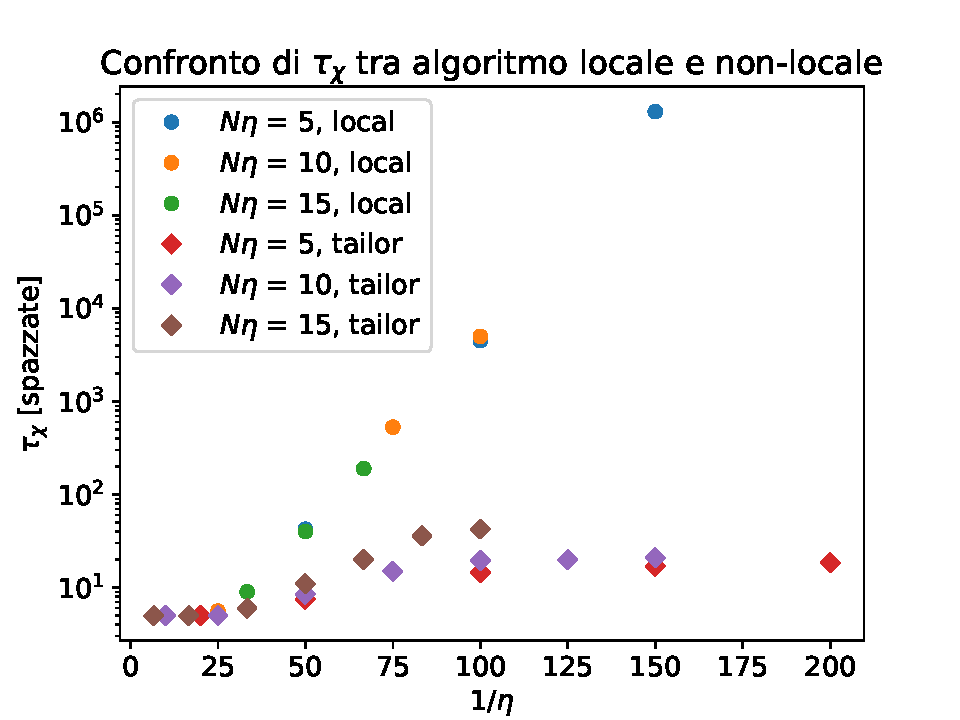
\includegraphics[width=10cm]{figure/csd_autocorr.pdf}
        \caption{Andamento del tempo di autocorrelazione $\tau_\chi$ della suscettività topologica nelle varie simulazioni effettuate. La ``coda'' per $N \to 0$ è dovuta al fatto che l'unità minima di tempo è data da 10 spazzate.}
        \label{fig:csd_autocorr}
    \end{figure}

    
    In figura \ref{fig:csd_autocorr} sono riportati i tempi di autocorrelazione di $\chi$ nelle varie simulazioni. Osserviamo che, qualitativamente, i valori di $\tau_\chi$ ottenuti dalle simulazioni con l'algoritmo locale si dispongono su un andamento grossomodo esponenziale, mentre quelli ottenuti dall'algoritmo non locale sembrano ``saturare'' ad un valore dipendente da $\beta$. Questa non è assolutamente un'analisi rigorosa, ma si può già vedere come l'algoritmo non-locale risolva in maniera efficiente il problema del critical slowing down esponenziale.
    
    \begin{figure}[htb]
        \centering
        \subfigure{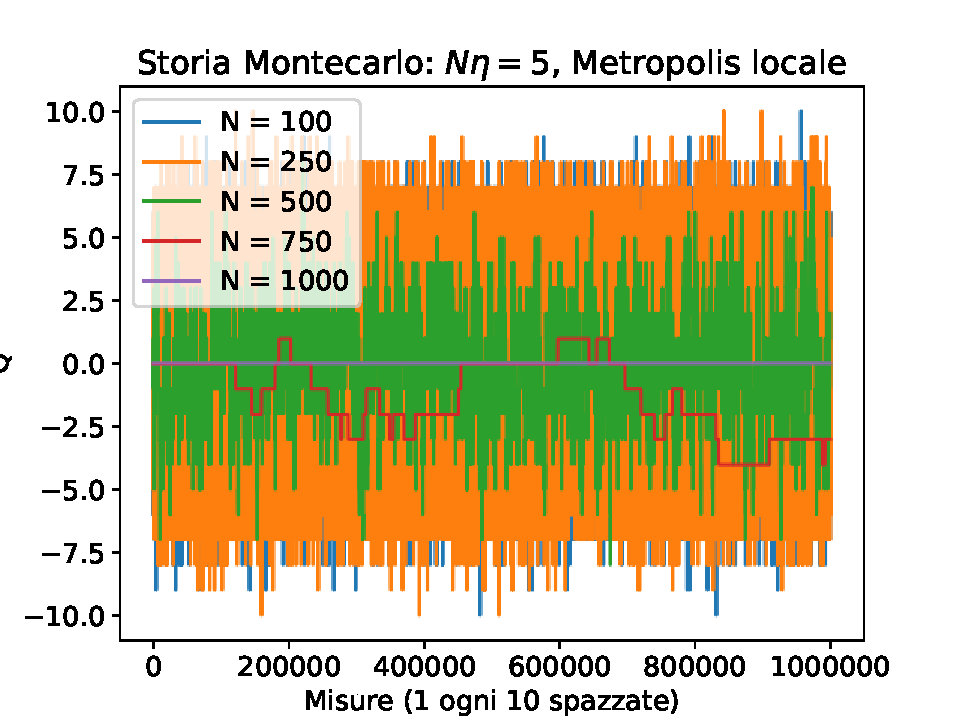
\includegraphics[width=7cm]{figure/csd_plot_local_5.pdf}}
        \subfigure{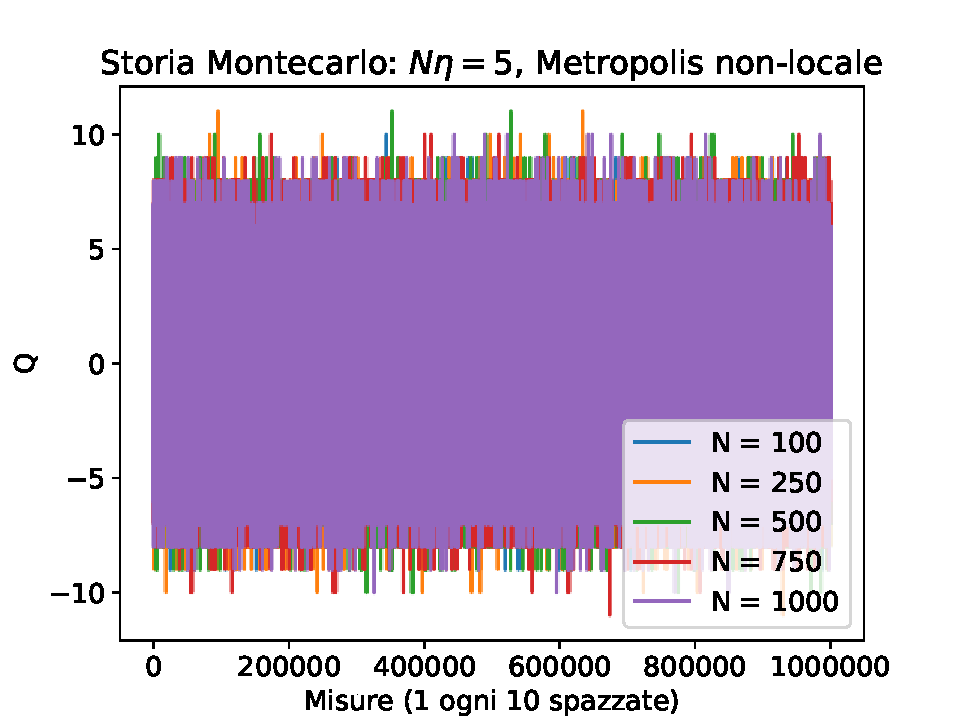
\includegraphics[width=7cm]{figure/csd_plot_tailor_5.pdf}}
        \caption{Congelamento dei modi topologici del sistema per $N\eta = 5$ al variare di N. Confronto con l'algoritmo non-locale.}
        \label{fig:csd_topfreezing}
    \end{figure}
    
    In figura \ref{fig:csd_topfreezing} possiamo vedere il confronto tra le storie Monte Carlo delle simulazioni fatte con l'algoritmo locale e l'algoritmo non locale, a $\beta = 5$. Notiamo che, con l'algoritmo locale, la carica topologica tende a fluttuare meno già per $N = 500$, A $N = 750$, la carica topologica cambia poche decine di volte in $10^6$ misure. A $N = 1000$, la carica topologica è completamente congelata a $Q = 0$. Nelle simulazioni fatte con l'algoritmo non locale, invece, il problema è completamente risolto: in tutte le simulazioni effettuate, $Q$ ``fluttua'' allo stesso modo.
    
    \subsection{Misura della suscettività topologica}
    
    Queste simulazioni sono state utilizzate per determinare la suscettività topologica del sistema per $\beta = 5, 10, 15$. Il valore teorico da confrontare è $\chi \to 1$ per $\beta \to \infty$.
    
    \section{Studio dello spettro e funzioni di correlazione}
    
    Poiché conosciamo già lo spettro del sistema, possiamo immediatamente dire che le osservabili $O_n \equiv a^n + {a^\dagger}^n$ connettono lo stato fondamentale con gli stati del livello energetico n-esimo.
    
    Di conseguenza, possiamo dire che, nel limite $\beta \to \infty$, 
    
    \begin{equation}
        C_n (\tau) \equiv \avg{ O_n(\tau)O_n(0) }_\beta - \avg{O_n}^2_\beta \sim A e^{-(E_n - E_0) \tau}
    \end{equation}
    
    Possiamo quindi calcolare il gap tra il livello n-esimo e il fondamentale studiando l'andamento delle funzioni di correlazione. 
    
    Questo non è di per sé particolarmente utile: abbiamo utilizzato il fatto che conosciamo già lo spettro del sistema! 
    
    Tuttavia, questo può essere usato come punto di partenza per studiare il sistema in presenza di un potenziale esterno (purché l'azione sia definita positiva). 

    
    \begin{equation}
         C_1 (\tau) \equiv \avg{\cos 2\pi x(\tau) \cos 2\pi x(0)}_\beta 
    \end{equation}
    \begin{equation}
        C_2 (\tau) \equiv \avg{\cos 4\pi x(\tau) \cos 4\pi x(0)}_\beta - \avg{\cos 4\pi x}^2_\beta
    \end{equation}
    
    \subsection{Primo livello}

    Sono state effettuate ... simulazioni con l'algoritmo non locale, con $\beta = 5$, $N = ...$, ognuna da $10^6$ misure, una ogni 10 spazzate.

    

    
\end{document}
